\section{Introduction}
In this chapter will be presented briefly the Kundera modular architecture, the way in which Kundera is supposed to be extended, the problems occurred in the process and how the community helped in achieving the result.
In section \ref{sec:kundera-datastore} are discussed the detail fo the extension for Google Datastore and in the section \ref{sec:kundera-table} the details for Azure Table.

\section{Overview of Kundera}
Kundera \cite{book:projpa2}{online:kundera} is an implementation for the JPA interface that now supports various NoSQL datastore. It supports by itself cross-datastore persistence in the sense that its allows an application to store and fetch data from different datastores.
Kundera provides all the code necessary to implement the JPA 2.1 standard interface independently from the underlying NoSQL database. In the \texttt{persistence.xml} configuration file is then possible to specify to Kundera what database is to be used for persistence.
The currently supported NoSQL databases are:
\begin{itemize}
\item Oracle NoSQL (versions 2.0.26 and 3.0.5)
\item HBase (version 0.94.3)
\item MongoDB (version 2.9.1)
\item Cassandra(versions1.2.9 and 2.0.4)
\item Redis (version 2.6.6)
\item Neo4j (version 1.8.1)
\item CouchDB (version 1.0.4)
\item Elastic Search (version 0.90.3)
\end{itemize}

Each of the supported databases has its own client implementation that uses a factory pattern, a Client- Factory is invoked to instantiate a Client which then use the database-specific API to interact with the underlying database.
The Client is invoked by Kundera-Core each time an operation has to be performed on the database. 

\begin{figure}[tbh]
  \centering
  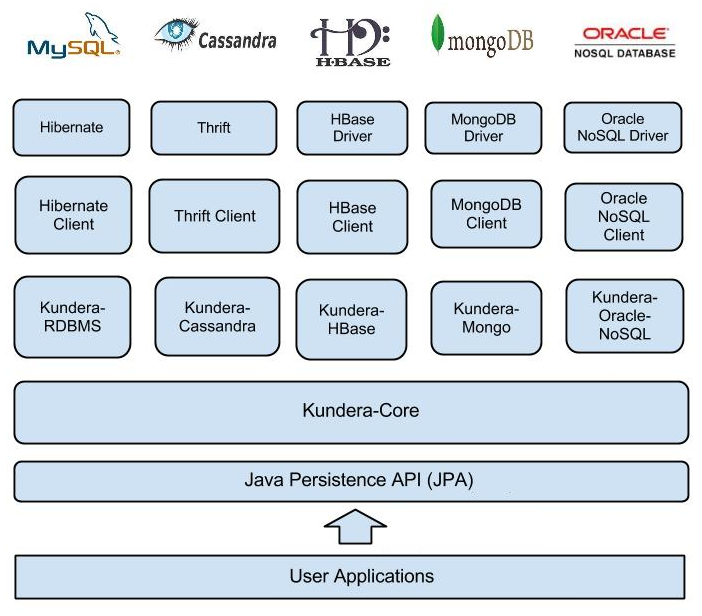
\includegraphics[scale=0.5]{images/kundera_architecture}
  \caption{Kundera architecture}
  \label{fig:kundera_architecture}
\end{figure}

The architecture of Kundera is shown in Figure \ref{fig:kundera_architecture}. The figure highlights the fact that the user application interacts with Kundera by exploiting the JPA interface. The Kundera-Core, in turn, interacts with the databases through the corresponding Clients.

\subsection{Kundera's Client Extension Framework}
Kundera as on open source project, thought that other developers could be interested in using it and extending its support to other datastore.
So in the wiki is presented the Client Extension Framework which provides a short description on how Kunders clients should work and provides the interfaces and classes that should be developed in order to make the client work properly.

Looking at Kundera architecture, is clear the modularity on which Kundera has been developed. When dealing with classes JPA annotated, the Kundera core provides the necessary logic to fully support the JPA 2.1 specification and when it's time to interact with the underlying database (for persisting, updating or reading entities) it delegate the operation to the configured client in the persistence.xml file.

The steps to build a new Kundera client, basically these are the blocks to be developed:
\begin{itemize}
\item the Client, which is the gateway to CRUD operations on database, except for queries;
\item the Client Factory, which is used by Kundera to instantiate the Client;
\item the Query implementor, which is used by Kundera to run JPA queries by invoking appropriate methods in Entity Readers;
\item the Entity Reader, which is used by Kundera to translate the queries into correct client
method calls;
\item optionally the Schema Manager, to support automatic schema generation.
\end{itemize}

\subsection{Approaching the extension}
It all seems quite simple but the problem is that the wiki is actually outdated. 
Two were the main problem in understaing what to do and how, firstly it turns out that the required interfaces are actualy a little different and also are the required methods
secondary, and slightly more time consuming, is that no hints are given on the structure and informations carried by the methods arguments.
The arguments carry data structures containing informations organized in the kundera metamodel which is the implementation of the JPA metamodel that contains all the information associated (throug annotations) to a class or a field.

Due to those problems and to shrink the developing time, the solution was to write on the Kundera google group page to ask the community for more updated infos about Kundera extension.
Briefly an answer has come and I've started a conversation with one of the developers of Kundera who helped me giving the updated infos for the Kundera's Client Extension Framework and tell me to look forward to the other client implementation for some examples. 
In light of the updated information it turns out that the Entity Reader was unnecessary and all the translation from JPA queries to datastore specific queries and their executions should be done in the Query Implementor.  

At this point since no answer were given about the Kundera metamodel, the most valid solution was to approach the extesion as a test driven development, so looking at the tests code of the other clients I've writed a set of unit tests one foreach feature (tests are analyzed in detail in chapter \ref{chap:eval}.
With the tests failing and the code of Kundera core was then possible to reverse engineer the arguments thath were not documented and thus be able to develop the new extensions.

\section{Developing client extension}
Has been developed two different extension for Kundera, the first one for Google Datastore and the second one for Azure Table.
After a first difficulty in figuring out how the extension have to be carried out, a main workflow has been the two projects have many parts in common. In the following sections the extensions are presented separately, the concepts are introduced the first time are encoutred and will be referenced further on if necessary specifying the differences, if any.

\subsection{Google App Engine Datastore client}
\label{sec:kundera-datastore}
The first extension that has been done is the one for Google App Engine (GAE) Datastore the NoSQL solution available in the App Engine runtime, is a key-value storage build on top of Google BigTable.

\subsubsection{JPA identifier}
Google Datastore is a key-value storage in which the most basic unit that can be stored is an Entity which is identified by a Key and composed of Properties.
Entities Keys contains various information about the entity itself:
\begin{itemize}
\item the entity Kind, which is used to group entities of the same type;
\item an entity identifier, used to distinguish entities of the same type;
\item an optional parent entity. 
\end{itemize}
Inspired by the Google JPA implementation on Datastore the idea was to use the Java class representing the datastore Key as indentifier for the POJO but unfortunately this is not possible since Kundera support only a well known set of Java datatypes.

The adopted solution is to handle the key internally, each time an opertion is required on Datastore the key relative to the entity is builded, the key Kind is directly mapped to the table name and the Key identifier is the user defined id in the @Id annotation.

IDs can be specified by the user or automatically generated, there are three possibilities:
\begin{itemize}
\item @Id annotation on a String type field
\item @Id annotation on a Long type field
\item @Id annotation on a long type field
\end{itemize}
For each case the ID can be user specified before the persist operation but in case of ID auto-generated the field must be of type String and the generated ID will be a string representation of a random java UUID.

Auto-geenerated ID are supported by Kundera thorugh @GeneratedValue with AUTO or TABLE strategy, only AUTO strategy is supported as a random Java UUID. It was not possible to use the Datastore API to generate ids since is necessary to know the Kind of the entity to be persisted but neither the AUTO strategy nor the TABLE one provides this infomation at generation time.

\subsubsection{Consistency}
In Datastore, entities are organized in Entity Groups based on their Ancestor Path, the ancestor path is a hierarchy containing the keys of the entities which are parents of the given one and thus are in the same entity group.

In Datastore consistency is managed through Entity Groups and so by defining the ancestor paths, entities within the same Entity Groups are managed in storng consistency, eventual consistency is used otherwise.

Datastore provide the possibility to create Ancestor path by defining them parent to other entities and is basically a task leaved to the user, no automated sorting or guessing is provided. Other wrapper around Datastore low-level API also leave this to the user, for example in Objectify the developer make use of an @Parent annotation that make the user able to specify the Ancestor Path.
Since JPA is well defined and adding such annotation will break the standard the only alternative way is trying to automatic guess the ancestor path.

Relationsips are clearly a good indicator when trying to guess if two entitiy kind can be hirearchically related:
\begin{itemize}
\item One to Many, since ther's a "many" side which is the non-owning side of the relationship the owning side can be clear used as parent for every entity in the "many" side;
\item Many to One, this is the inverse of the previous type and thus entities sould be already organized;
\item One to One, can be treated like the One to Many
\item Many to Many, in this case since there's a join table between the entities there are several solutions:
\begin{itemize}
\item put the join table and the non-owning entities parent to the owning ones;
\item put all the join table, the entities on the owning side and the ones on the non-owning side under a common fictitious root entity kind
\end{itemize}
\end{itemize}

This unfourtanently is not conventien since there's lot of possibilities, thinks for the Many to Many case but more important is that if an entity is in more than one on those relationships is not possible to prioritize them and choose unless asking to the user which is the case, furthermore when declaring a entity parent to another is always necessary to know the Key of the parent beside the Key of the entity itself to be able to retrieve it from Datastore and as Kundera is structured this kind of information is not available in the client but must be serached inside the kundera metadata when possible.

For those reasons was not possible without causing strange behaviours, automatically guess the Ancestor Paths through JPA relationships so at the end is not possible for the user to manage entity consistency, each entity is stored in a separated entity group identified by its Kind (the name of the JPA table associated to the entity).

\subsubsection{JPA relationships}
All the JPA supported relationships has been implemented in the client has been implemented like they would be in a RDBMS system.
So for One to One and One to Many relationships, where on the onwer side of the relationships there's a link to the non-owning side, the connection is keeped persisting within the entity the Key (Kind and identified) of the related entity.

For the Many to One relationships there would be to solutions:
\begin{itemize}
\item persist a list of Key of the related entities;
\item do not persist anything within the entity but fill the relationship with a query.
\end{itemize}
The second solution has been adopted since more consistent with the other client implementation and with the classic implementation of the relation type for RDBMS.

For the Many to Many relationships a join table is created based on the directives of the user specified in the annotations, then is filled each time one entity is persisted and is related with another one through a many to many relationship.

\subsection{Queries}
Here there's a comparative table for the JPQL operator suppoted:
\begin{table}[h]
\begin{tabular}{|l|c|}
\hline
\textbf{JPA-QL Clause} & \textbf{Datastore support} \\ \hline\hline
\textit{SELECT}        & yes \\ \hline
\textit{UPDATE}        & yes \\ \hline
\textit{DELETE}        & yes \\ \hline
\textit{ORDER BY}      & yes \\ \hline
\textit{AND}           & yes \\ \hline
\textit{OR}            & yes \\ \hline
\textit{BETWEEN}       & yes \\ \hline
\textit{LIKE}          & no  \\ \hline
\textit{IN}            & yes  \\ \hline
\textit{=}             & yes \\ \hline
\textit{\textgreater}  & yes \\ \hline
\textit{\textless}     & yes \\ \hline
\textit{\textgreater=} & yes \\ \hline
\textit{\textless=}    & yes \\ \hline
\end{tabular}
\end{table}

\subsubsection{Embedded entities}
For JPA embedded entities eh implementation for Datastore is straightforward because its supports natively embedded entities.

The implementation so make use of this feature translating the embedded POJO in a Datastore embedded Entity and then persist it within the parent entity.

\subsubsection{Collection fields}
Collections and maps are natively supported by datastore but are supported only if composed of primitives Java datatypes, to be able to save whatever kind of collection or map independently by the datatype thath compose it, the collection or map itself is serialized when persisted and deserialized when readed.

Serialization and deserialization is completely handled into the extension making it completely transparent to the user.

\subsubsection{Enumeration fields}
Enum fields are supported simply by persisting its string represention and instantiating the enum type bak when the entity is read.

\subsubsection{Schema Manager}
Schema manager as required by Kundera has to exploit four cases:
\begin{itemize}
\item validate which validates schema tables based on entity definition.
\item update which updates schema tables based on entity definition.
\item create which schema tables based on entity definitions.
\item create\textunderscore drop which drops (if exists) schema, then creates schema tables based on entity definitions.
\end{itemize}
The first two cases are quite useless for a Datastore since ther'se no fixed schema for entities, entities with same Kind can have different Properties withouth restriction.
Also the "create" case is usless for Datastore since if a new entity of an unknown Kind is persisted it's created withoud the need to explicitly define it first as a "table".
The remanining case "create\textunderscore drop" will so just drop the current schema deleting all the entities af all the Kinds without recreating schema since it construct by itself.

\subsection{Azure Table client}
\label{sec:kundera-table}
Table is the NoSQL solution developed by Microsoft, is a key-value storage and it's available inside Azure environment.

\subsubsection{JPA identifier}
In Azure Table an entity is identified by the pair partition key and row key 

\subsubsection{Consistency}
In Azure Table strong consistency is guaranteed while entities are stored within the same partition key otherwise consistency will be eventual. IDs are supported only in field of type String (so only a String field can be annotated with @Id). User can define IDs both with or without partition key.

\subsubsection{Define both row key and partition key}
This can be done in two ways:
\begin{itemize}
\item using AzureTableKey.asString method by passing both partition key and row key to obtain a string representation of the whole key and assign it to the entity ID field before persist.
\item manually define the entity ID before persist the entity, the string must follow the pattern partitionKey\textunderscore rowKey.
\end{itemize}

\subsubsection{Define only the row key}
If only the row key is defined, the partition key is implicitly the default one (which can be set in a datastore specific properties file).

There are three ways to do this:
\begin{itemize}
\item auto-generated IDs (the row key is a random java UUID)
\item manually define the entity ID before persist the entity
\item using AzureTableKey.asString passing as parameter the desired row key and assign its result to the entity ID field before persist.
\end{itemize}

\subsubsection{JPA relationships}
Also for Azure Table, to keep uniform the extension behaviour, all the JPA supported relationships has been implemented in the client has been implemented like they would be in a RDBMS system.

The only difference is that when is needed to keep a reference to another entity in the owning side of a relationship is persisted within the entity the partition key and the row key of the related entity since the pair partition key and row key universally identify an entity.

\subsection{Queries}
Here there's a comparative table for the JPQL operator suppoted:
\begin{table}[h]
\begin{tabular}{|l|c|}
\hline
\textbf{JPA-QL Clause} & \textbf{Table support} \\ \hline\hline
\textit{SELECT}        & yes \\ \hline
\textit{UPDATE}        & yes \\ \hline
\textit{DELETE}        & yes \\ \hline
\textit{ORDER BY}      & no \\ \hline
\textit{AND}           & yes \\ \hline
\textit{OR}            & yes \\ \hline
\textit{BETWEEN}       & yes \\ \hline
\textit{LIKE}          & no  \\ \hline
\textit{IN}            & no  \\ \hline
\textit{=}             & yes \\ \hline
\textit{\textgreater}  & yes \\ \hline
\textit{\textless}     & yes \\ \hline
\textit{\textgreater=} & yes \\ \hline
\textit{\textless=}    & yes \\ \hline
\end{tabular}
\end{table}

\subsubsection{Embedded entities}
Embedded fields are not supported natively by Azure Table so the solution adopted is to serialize the field annotated as embedded to be able to ave it to the storage and deserializing it when the entity is read.

\subsubsection{Collection fields}
Collection and maps are not supported by Azure Table since it supports only a set of primitive Java datatypes.
To support even complex collection or maps the solution is, like Datastore, serialize the entire collection or map when persisting the entity and deserializing it when reading the entity from the storage.

\subsubsection{Enumeration fields}
Enum fields are supported simply by persisting its string represention and instantiating the enum type bak when the entity is read.

\subsubsection{Schema Manager}
Schema manager as required by Kundera has to exploit four cases:
\begin{itemize}
\item validate which validates schema tables based on entity definition.
\item update which updates schema tables based on entity definition.
\item create which schema tables based on entity definitions.
\item create\textunderscore drop which drops (if exists) schema, then creates schema tables based on entity definitions.
\end{itemize}
Here, like Google Datastore, the first two cases are quite useless for Azure Table since ther'se no fixed schema and entities within the same Table can have different properties withouth restriction.

Azure Table need that the Table in which entities are stored exists before trying to create entities so the "create" case simply iterate over all table names and creates it in the database. 
For the "create\textunderscore drop" case, all tables are dropped (and so all the contained entities) and re-created.

\section{Summary}
In this chpater has been introduced in details how Kundera extension should been developed, the problem encountered during the development, how tey've been addressed and the detail of the implementation of the two extensions including what the feature currently supported.
In the next chapter will be explained how has been possible to integrate Kundera into CPIM as part of the NoSQL service.
